%===============================================================================
% LaTeX sjabloon voor de bachelorproef toegepaste informatica aan HOGENT
% Meer info op https://github.com/HoGentTIN/latex-hogent-report
%===============================================================================

\documentclass[dutch,dit,thesis]{hogentreport}

% TODO:
% - If necessary, replace the option `dit`' with your own department!
%   Valid entries are dbo, dbt, dgz, dit, dlo, dog, dsa, soa
% - If you write your thesis in English (remark: only possible after getting
%   explicit approval!), remove the option "dutch," or replace with "english".

\usepackage{lipsum} % For blind text, can be removed after adding actual content

%% Pictures to include in the text can be put in the graphics/ folder
\graphicspath{{../graphics/}}

%% For source code highlighting, requires pygments to be installed
%% Compile with the -shell-escape flag!
%% \usepackage[chapter]{minted}
%% If you compile with the make_thesis.{bat,sh} script, use the following
%% import instead:
\usepackage[chapter,outputdir=../output]{minted}
\usemintedstyle{solarized-light}

%% Formatting for minted environments.
\setminted{%
    autogobble,
    frame=lines,
    breaklines,
    linenos,
    tabsize=4
}

%% Ensure the list of listings is in the table of contents
\renewcommand\listoflistingscaption{%
    \IfLanguageName{dutch}{Lijst van codefragmenten}{List of listings}
}
\renewcommand\listingscaption{%
    \IfLanguageName{dutch}{Codefragment}{Listing}
}
\renewcommand*\listoflistings{%
    \cleardoublepage\phantomsection\addcontentsline{toc}{chapter}{\listoflistingscaption}%
    \listof{listing}{\listoflistingscaption}%
}

% Other packages not already included can be imported here

%%---------- Document metadata -------------------------------------------------
% TODO: Replace this with your own information
\author{Thomas Vanderveken}
\supervisor{TBD}
\cosupervisor{TBD}
\title[Optionele ondertitel]%
    {Titel TBD}
\academicyear{\advance\year by -1 \the\year--\advance\year by 1 \the\year}
\examperiod{3}
\degreesought{\IfLanguageName{dutch}{Professionele bachelor in de toegepaste informatica}{Bachelor of applied computer science}}
\partialthesis{false} %% To display 'in partial fulfilment'
%\institution{Internshipcompany BVBA.}

%% Add global exceptions to the hyphenation here
\hyphenation{back-slash}

%% The bibliography (style and settings are  found in hogentthesis.cls)
\addbibresource{bachproef.bib}            %% Bibliography file
\addbibresource{../voorstel/voorstel.bib} %% Bibliography research proposal
\defbibheading{bibempty}{}

%% Prevent empty pages for right-handed chapter starts in twoside mode
\renewcommand{\cleardoublepage}{\clearpage}

\renewcommand{\arraystretch}{1.2}

%% Content starts here.

\begin{document}

%---------- Front matter -------------------------------------------------------

\frontmatter

\hypersetup{pageanchor=false} %% Disable page numbering references
%% Render a Dutch outer title page if the main language is English
\IfLanguageName{english}{%
    %% If necessary, information can be changed here
    \degreesought{Professionele Bachelor toegepaste informatica}%
    \begin{otherlanguage}{dutch}%
       \maketitle%
    \end{otherlanguage}%
}{}

%% Generates title page content
\maketitle
\hypersetup{pageanchor=true}

%%=============================================================================
%% Voorwoord
%%=============================================================================

\chapter*{\IfLanguageName{dutch}{Woord vooraf}{Preface}}%
\label{ch:voorwoord}

%% TODO:
%% Het voorwoord is het enige deel van de bachelorproef waar je vanuit je
%% eigen standpunt (``ik-vorm'') mag schrijven. Je kan hier bv. motiveren
%% waarom jij het onderwerp wil bespreken.
%% Vergeet ook niet te bedanken wie je geholpen/gesteund/... heeft

\lipsum[1-2]
%%=============================================================================
%% Samenvatting
%%=============================================================================

% TODO: De "abstract" of samenvatting is een kernachtige (~ 1 blz. voor een
% thesis) synthese van het document.
%
% Een goede abstract biedt een kernachtig antwoord op volgende vragen:
%
% 1. Waarover gaat de bachelorproef?
% 2. Waarom heb je er over geschreven?
% 3. Hoe heb je het onderzoek uitgevoerd?
% 4. Wat waren de resultaten? Wat blijkt uit je onderzoek?
% 5. Wat betekenen je resultaten? Wat is de relevantie voor het werkveld?
%
% Daarom bestaat een abstract uit volgende componenten:
%
% - inleiding + kaderen thema
% - probleemstelling
% - (centrale) onderzoeksvraag
% - onderzoeksdoelstelling
% - methodologie
% - resultaten (beperk tot de belangrijkste, relevant voor de onderzoeksvraag)
% - conclusies, aanbevelingen, beperkingen
%
% LET OP! Een samenvatting is GEEN voorwoord!

%%---------- Nederlandse samenvatting -----------------------------------------
%
% TODO: Als je je bachelorproef in het Engels schrijft, moet je eerst een
% Nederlandse samenvatting invoegen. Haal daarvoor onderstaande code uit
% commentaar.
% Wie zijn bachelorproef in het Nederlands schrijft, kan dit negeren, de inhoud
% wordt niet in het document ingevoegd.

\IfLanguageName{english}{%
\selectlanguage{dutch}
\chapter*{Samenvatting}

\selectlanguage{english}
}{}

%%---------- Samenvatting -----------------------------------------------------
% De samenvatting in de hoofdtaal van het document

\chapter*{\IfLanguageName{dutch}{Samenvatting}{Abstract}}


Deze bachelorproef onderzoekt de toepassing van Tekst mining, AI en NLP- technologieën om gegevens uit pre-2013 SEC 13F-meldingen te extraheren, te standaardiseren en te integreren in een gestructureerde databank. Het onderzoek werd gestructureerd in verschillende fasen, te beginnen met het formuleren van een centrale onderzoeksvraag, gevolgd door een uitgebreide literatuurstudie om de uitdagingen van 13F-meldingen te begrijpen en de mogelijkheden van AI in deze context te verkennen. Vervolgens werd een methodologie ontwikkeld, waarbij duidelijke eisen werden gesteld aan de proof of concept (POC).

In de POC werd regex gebruikt om gestructureerde data uit de headers van de 13F-rapporten efficiënt te extraheren, terwijl het Llama 3.18B-model werd getraind en ingezet om tabelgegevens te extraheren en te standaardiseren. De implementatie toonde aan dat het mogelijk is om AI voor deze taken in te zetten, maar onthulde ook beperkingen als gevolg van beperkte trainingsdata en rekenkracht, wat de prestaties van het model op niet-standaard gevallen beïnvloedde. De bevindingen suggereren dat, hoewel AI-technieken veelbelovend zijn, verdere verfijning en opschaling nodig zijn voor bredere toepassing.

Uiteindelijk vormt dit onderzoek een sterke basis voor toekomstig werk, waaronder het mogelijke gebruik van geavanceerdere modellen zoals GPT en het verkennen van andere bestandstypen. De studie benadrukt het significante potentieel van AI om de verwerking en analyse van historische financiële gegevens te verbeteren, wat de weg vrijmaakt voor efficiënter gegevensbeheer en verbeterde voorspellende modellen.

De meerwaarde van dit onderzoek is vooral relevant voor financiële instellingen, onderzoekers en data-analisten die werken met historische financiële gegevens, met name die van de SEC 13F-meldingen. Door de ontwikkeling van een proof of concept die aantoont dat AI-technologieën zoals NLP en machine learning effectief kunnen worden ingezet voor het standaardiseren en integreren van dergelijke gegevens, biedt dit onderzoek inzichten en tools die de efficiëntie en nauwkeurigheid van gegevensverwerking aanzienlijk kunnen verbeteren.

%---------- Inhoud, lijst figuren, ... -----------------------------------------

\tableofcontents

% In a list of figures, the complete caption will be included. To prevent this,
% ALWAYS add a short description in the caption!
%
%  \caption[short description]{elaborate description}
%
% If you do, only the short description will be used in the list of figures

\listoffigures

% If you included tables and/or source code listings, uncomment the appropriate
% lines.
\listoftables

\listoflistings

% Als je een lijst van afkortingen of termen wil toevoegen, dan hoort die
% hier thuis. Gebruik bijvoorbeeld de ``glossaries'' package.
% https://www.overleaf.com/learn/latex/Glossaries

%---------- Kern ---------------------------------------------------------------

\mainmatter{}

% De eerste hoofdstukken van een bachelorproef zijn meestal een inleiding op
% het onderwerp, literatuurstudie en verantwoording methodologie.
% Aarzel niet om een meer beschrijvende titel aan deze hoofdstukken te geven of
% om bijvoorbeeld de inleiding en/of stand van zaken over meerdere hoofdstukken
% te verspreiden!

%%=============================================================================
%% Inleiding
%%=============================================================================

\chapter{\IfLanguageName{dutch}{Inleiding}{Introduction}}%
\label{ch:inleiding}

Regelgevende filings die door institutionele beleggers, zoals pensioenfondsen en vermogensbeheerders worden ingediend, bieden belangrijke inzichten in marktpatronen en beleggingsstrategie. De 13F-meldingen die worden ingediend bij de Amerikaanse Securities and Exchange Commission (SEC) zijn een van de belangrijkste bronnen van deze informatie. Deze registraties geven informatie weer over de bezittingen van institutionele beleggers, waardoor ze van cruciaal belang zijn voor het uitvoeren van financieel onderzoek en het analyseren van beleggingen. 13F-meldingen van voor 2013 leveren echter aanzienlijke problemen op vanwege hun variabele vormen en structuren, die de menselijke verwerking en analyse complexer maken.
De opkomst van geavanceerde AI-technologie biedt een potentiële kans om deze problemen aan te pakken. Natural Language Processing (NLP) en Machine Learning (ML) bieden geavanceerde technieken aan voor het extraheren en organiseren van gegevens uit tekst zonder vooraf gedefinieerde structuur. Door gebruik te maken van deze technologieën is het mogelijk om het proces van het standaardiseren en combineren van eerdere 13F meldingen in een goed georganiseerde relationele databank te automatiseren, waardoor de toegang en het gebruik wordt verbeterd.

Het doel van dit proefschrift is het creëren van een proof-of-concept toepassing die Natural Language Processing (NLP) en Machine Learning (ML) technieken gebruikt om 13F aanvragen van voor 2013 te standaardiseren en te integreren in een relationele databank. Het voorgestelde systeem is gericht op het stroomlijnen van het gegevens extractieproces door de meldingen automatisch om te zetten in een gestandaardiseerd formaat met een hoge efficiëntie en nauwkeurigheid. Dit zou niet alleen de analyse van financiële gegevens uit het verleden optimaliseren, maar ook het werk en de kosten verminderen die gepaard gaan met handmatige gegevensverwerking.

Bovendien zouden de gestandaardiseerde gegevens het begrip van investeringspatronen uit het verleden verbeteren en het creëren van voorspellingsmodellen ondersteunen. Het onderzoek zal beginnen met een uitgebreide literatuurstudie om de meest efficiënte Natural Language Processing (NLP) en Machine Learning (ML) strategieën voor dit specifiek doel te bepalen. Daarna zal een proof-of-concept toepassing worden gecreëerd en beoordeeld worden op nauwkeurigheid, efficiëntie en bruikbaarheid.

De inleiding geeft een beknopt overzicht van de redenen, doelen en het belang van het onderzoek weer. Dit werk wil een nuttige bijdrage leveren aan de analyse van financiële gegevens en onderzoekers en analisten een nuttig hulpmiddel bieden door de moeilijkheden aan te pakken die gepaard gaan met het verwerken van oudere 13F-meldingen.

\section{\IfLanguageName{dutch}{Probleemstelling}{Problem Statement}}%
\label{sec:probleemstelling}

13F meldingen van de SEC voor 2013, zijn belangrijke bestanden voor financieel onderzoek, ze bevatten namelijk data over de stocks dat investment managers beheren. Maar deze zijn vaak inconsistent in opmaak en moeilijker toegankelijk, wat manuele analyse bemoeilijkt. Er ontbreekt namelijk een geautomatiseerd systeem om deze gegevens te standaardiseren en in een databank te integreren. Dit bemoeilijkt de opportuniteiten voor diepgaande analyses en het verkrijgen van inzichten in beleggingstrends.

\section{\IfLanguageName{dutch}{Onderzoeksvraag}{Research question}}%
\label{sec:onderzoeksvraag}

Hoe kunnen AI-technologieën zoals Natural Language Processing (NLP) en Machine Learning (ML) effectief worden toegepast om 13F-meldingen van de SEC van vóór 2013 te standaardiseren en te integreren in een gestructureerde databank, zodat de historische gegevens efficiënter kunnen worden geanalyseerd en vergeleken?


\section{\IfLanguageName{dutch}{Onderzoeksdoelstelling}{Research objective}}%
\label{sec:onderzoeksdoelstelling}

Het hoofddoel van dit onderzoek is het ontwikkelen van een geautomatiseerde methode die gebruikmaakt van AI-technologieën, zoals NLP en ML, om de data uit de 13F meldingen van voor 2013 te extraheren, standaardiseren en te integreren in een relationele databank. Dit moet leiden tot een efficiëntere en meer accurate extractie van gegevens uit deze documenten, waardoor de toegankelijkheid en bruikbaarheid van de data voor financieel onderzoek en investeringsanalyse aanzienlijk worden verbeterd. 


\section{\IfLanguageName{dutch}{Opzet van deze bachelorproef}{Structure of this bachelor thesis}}%
\label{sec:opzet-bachelorproef}

% Het is gebruikelijk aan het einde van de inleiding een overzicht te
% geven van de opbouw van de rest van de tekst. Deze sectie bevat al een aanzet
% die je kan aanvullen/aanpassen in functie van je eigen tekst.

Het verdere verloop van deze bachelorproef is opgebouwd als volgt:

In Hoofdstuk~\ref{ch:stand-van-zaken} wordt een overzicht gegeven van de stand van zaken binnen het onderzoeksdomein, op basis van een literatuurstudie.

In Hoofdstuk~\ref{ch:methodologie} wordt de methodologie toegelicht en worden de gebruikte onderzoekstechnieken besproken om een antwoord te kunnen formuleren op de onderzoeksvragen.

In Hoofdstuk~\ref{ch:methodologie}  wordt de proof-of-concept besproken. De inhoud omvat de ingewikkelde technische specificaties, structuur en tools, samen met de functionele elementen zoals de modellen en de databank.

% TODO: Vul hier aan voor je eigen hoofstukken, één of twee zinnen per hoofdstuk

In Hoofdstuk~\ref{ch:conclusie}, tenslotte, wordt de conclusie gegeven en een antwoord geformuleerd op de onderzoeksvragen. Daarbij wordt ook een aanzet gegeven voor toekomstig onderzoek binnen dit domein.
\chapter{\IfLanguageName{dutch}{Stand van zaken}{State of the art}}%
\label{ch:stand-van-zaken}

% Tip: Begin elk hoofdstuk met een paragraaf inleiding die beschrijft hoe
% dit hoofdstuk past binnen het geheel van de bachelorproef. Geef in het
% bijzonder aan wat de link is met het vorige en volgende hoofdstuk.

% Pas na deze inleidende paragraaf komt de eerste sectiehoofding.

Dit hoofdstuk bevat je literatuurstudie. De inhoud gaat verder op de inleiding, maar zal het onderwerp van de bachelorproef *diepgaand* uitspitten. De bedoeling is dat de lezer na lezing van dit hoofdstuk helemaal op de hoogte is van de huidige stand van zaken (state-of-the-art) in het onderzoeksdomein. Iemand die niet vertrouwd is met het onderwerp, weet nu voldoende om de rest van het verhaal te kunnen volgen, zonder dat die er nog andere informatie moet over opzoeken \autocite{Pollefliet2011}.

Je verwijst bij elke bewering die je doet, vakterm die je introduceert, enz.\ naar je bronnen. In \LaTeX{} kan dat met het commando \texttt{$\backslash${textcite\{\}}} of \texttt{$\backslash${autocite\{\}}}. Als argument van het commando geef je de ``sleutel'' van een ``record'' in een bibliografische databank in het Bib\LaTeX{}-formaat (een tekstbestand). Als je expliciet naar de auteur verwijst in de zin (narratieve referentie), gebruik je \texttt{$\backslash${}textcite\{\}}. Soms is de auteursnaam niet expliciet een onderdeel van de zin, dan gebruik je \texttt{$\backslash${}autocite\{\}} (referentie tussen haakjes). Dit gebruik je bv.~bij een citaat, of om in het bijschrift van een overgenomen afbeelding, broncode, tabel, enz. te verwijzen naar de bron. In de volgende paragraaf een voorbeeld van elk.

\textcite{Knuth1998} schreef een van de standaardwerken over sorteer- en zoekalgoritmen. Experten zijn het erover eens dat cloud computing een interessante opportuniteit vormen, zowel voor gebruikers als voor dienstverleners
 op vlak van informatietechnologie~\autocite{Creeger2009}.

Let er ook op: het \texttt{cite}-commando voor de punt, dus binnen de zin. Je verwijst meteen naar een bron in de eerste zin die erop gebaseerd is, dus niet pas op het einde van een paragraaf.


\begin{figure}
  \centering
  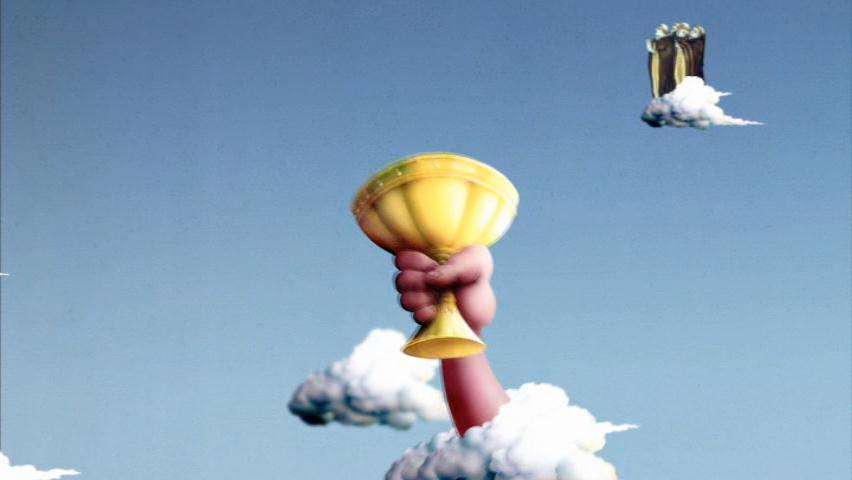
\includegraphics[width=0.8\textwidth]{grail.jpg}
  \caption[Voorbeeld figuur.]{\label{fig:grail}Voorbeeld van invoegen van een figuur. Zorg altijd voor een uitgebreid bijschrift dat de figuur volledig beschrijft zonder in de tekst te moeten gaan zoeken. Vergeet ook je bronvermelding niet!}
\end{figure}

\begin{listing}
  \begin{minted}{python}
    import pandas as pd
    import seaborn as sns

    penguins = sns.load_dataset('penguins')
    sns.relplot(data=penguins, x="flipper_length_mm", y="bill_length_mm", hue="species")
  \end{minted}
  \caption[Voorbeeld codefragment]{Voorbeeld van het invoegen van een codefragment.}
\end{listing}


\begin{table}
  \centering
  \begin{tabular}{lcr}
    \toprule
    \textbf{Kolom 1} & \textbf{Kolom 2} & \textbf{Kolom 3} \\
    $\alpha$         & $\beta$          & $\gamma$         \\
    \midrule
    A                & 10.230           & a                \\
    B                & 45.678           & b                \\
    C                & 99.987           & c                \\
    \bottomrule
  \end{tabular}
  \caption[Voorbeeld tabel]{\label{tab:example}Voorbeeld van een tabel.}
\end{table}




% ----------------------------------------------------------------------------
Het 13F formulier van de Securities and Exchange Commission (SEC) is een rapport dat institutionele vermogensbeheerders elk kwartaal moeten indienen als ze voor meer dan \$100 miljoen of meer aan Section 13(f) effecten bezitten. Sectie 13(f) van de Securities Exchange Act van 1934 legt deze verplichting op met als doel de transparantie van het effectenbezit van grote institutionele beleggers te vergroten. In 1975 implementeerde het Congres deze bepaling om de toegankelijkheid van informatie over de investeringsactiviteiten van deze bedrijven te verbeteren. Ze geloofden dat dit openbaarmakingsprogramma het vertrouwen van beleggers in de integriteit van de effectenmarkten van de Verenigde Staten zou versterken~\autocite(SECform13F2024).\\
Formulier 13F biedt een uitgebreid overzicht van de aandelenbeleggingen van prominente beleggingsentiteiten wereldwijd, waardoor het een uiterst belangrijk hulpmiddel is voor analisten, onderzoekers en beleggers die inzicht willen krijgen in markttrends en de beleggingsbenaderingen van belangrijke marktspelers. Het onverwerkte tekstuele formaat waarin deze inzendingen worden aangeleverd, vormt echter een aanzienlijke belemmering voor effectieve gegevensextractie en -analyse.\\
Kunstmatige intelligentie (AI) en Machine Learning (ML) technologieën hebben de extractie en organisatie van gegevens uit ongestructureerde tekst de afgelopen jaren aanzienlijk veranderd. Geavanceerde methodologieën zoals Natural Language Processing (NLP) en deep learning modellen maken het mogelijk om tekstuele 13F aanvragen om te zetten in gestructureerde datasets die geschikt zijn voor grondige analyse en studie. Vervolgens kunnen deze georganiseerde gegevens worden opgeslagen in databases, zodat ze eenvoudiger kunnen worden opgevraagd, weergegeven en onderzocht.\\
\\
Het doel van deze literatuurstudie is het onderzoeken en beoordelen van de verschillende Artificial Intelligence (AI) en Machine Learning (ML) technieken die kunnen worden gebruikt om gegevens uit 13F-formulieren te extraheren, te organiseren en op te slaan. Het doel van het onderzoek is het bepalen van de meest efficiënte methoden om de ongeorganiseerde inhoud van deze documenten om te zetten in een gestructureerd formaat dat geschikt is voor analyse en opslag in een database. Dit houdt in dat er een vergelijkend onderzoek wordt gedaan naar verschillende kunstmatige intelligentie methodologieën, zoals Natural Language Processing (NLP) en Deep Learning modellen, en dat bepaalde tools zoals BERT, GPT en SpaCy worden geëvalueerd. De evaluatie zal ook de integratie van gestructureerde gegevens in databasemanagementsystemen (DBMS) onderzoeken, om te garanderen dat de geëxtraheerde gegevens gemakkelijk beschikbaar zijn voor later onderzoek en analyse. Het doel van deze evaluatie is om een uitgebreide kennis te krijgen van de meest effectieve procedures en technologie voor het verwerken van 13F-formulieren. 

% ----------------------------------------------------------------------------
\section{AI- en Tekstextractietechnieken}
\subsection{Natural Language Processing (NLP)}
\subsection{Machine Learning (ML) benaderingen}
% ----------------------------------------------------------------------------
\subsection{Vergelijkende analuyse van techologiën}
To be reviewed
% ----------------------------------------------------------------------------
\section{Technieken en Tools}
\subsection{Tekstverwerkingtools}
\subsection{Database Management Systemen (DBMS)}
\subsection{ETL Tools}
% ----------------------------------------------------------------------------
\section{Uitdagingen en beperkingen}
\subsection{Camplexiteit van financiële Tekst}
\subsection{Gegevenskwaliteit en Validatie}
\subsection{Databaseprestaties}
% ----------------------------------------------------------------------------
\section{Leemtes in huidig onderzoek}
\subsection{Onbehandelde kwesties}
\subsection{Verbeteringsmogelijkehden}

% ----------------------------------------------------------------------------
\section{Toekomstige richtingen}
\subsection{Voortgang in AI en NLP}
\subsection{Integration with financiele analyse}
% ----------------------------------------------------------------------------
\section{conclusie}
\subsection{Samenvatting van Bevindingen}
\subsection{Implicaties van het onderzoek}
%%=============================================================================
%% Methodologie
%%=============================================================================

\chapter{\IfLanguageName{dutch}{Methodologie}{Methodology}}%
\label{ch:methodologie}

%% TODO: In dit hoofstuk geef je een korte toelichting over hoe je te werk bent
%% gegaan. Verdeel je onderzoek in grote fasen, en licht in elke fase toe wat
%% de doelstelling was, welke deliverables daar uit gekomen zijn, en welke
%% onderzoeksmethoden je daarbij toegepast hebt. Verantwoord waarom je
%% op deze manier te werk gegaan bent.
%% 
%% Voorbeelden van zulke fasen zijn: literatuurstudie, opstellen van een
%% requirements-analyse, opstellen long-list (bij vergelijkende studie),
%% selectie van geschikte tools (bij vergelijkende studie, "short-list"),
%% opzetten testopstelling/PoC, uitvoeren testen en verzamelen
%% van resultaten, analyse van resultaten, ...
%%
%% !!!!! LET OP !!!!!
%%
%% Het is uitdrukkelijk NIET de bedoeling dat je het grootste deel van de corpus
%% van je bachelorproef in dit hoofstuk verwerkt! Dit hoofdstuk is eerder een
%% kort overzicht van je plan van aanpak.
%%
%% Maak voor elke fase (behalve het literatuuronderzoek) een NIEUW HOOFDSTUK aan
%% en geef het een gepaste titel.

\lipsum[21-25]


%%=============================================================================
%% Methodologie
%%=============================================================================

\chapter{\IfLanguageName{dutch}{Benodigdheden}{Needs}}%
\label{ch:benodigdheden}

%
%\section{Must Have}
%\begin{enumerate}
%    \item De gekozen tools en resources moeten gratis toegankelijk zijn.
%    \item Model of script voor header extractie
%    \item Model of script voor het extraheren van tabel data uit de text bestanden
%    \item Databank om ge-extraheerde data in op te slagen.
%
%\end{enumerate}
%
%
%\section{Should Have}
%    \item Script dat de data (13F-meldingen) download van de SEC en voorbereid op data extractie
%    \item Databank om ge-extraheerde data in op te slagen.
%    \item Er moet gebruik worden gemaakt van open-source software of diensten met een volledig gratis licentie, zoals GNU General Public License (GPL), MIT-licentie, of soortgelijke. Er mogen geen verborgen kosten of verplichtingen zijn verbonden aan het gebruik van deze software of diensten.
%      
%  
%
%
%\section{Won't Have}
%\begin{enumerate}
%    \item  Het ontwikkelen van een centrale interface voor het maken van een dashboard of vergelijkbare functionaliteiten.
%    \item Betalende technieken
%\end{enumerate}
Dit hoofdstuk van deze bachelorproef bespreekt de vereisten voor de ontwikkeling van de proof of concept. De lijst van benodigdheden is opgesteld volgens de MoSCoW-methode, waarmee duidelijk kan worden bepaald wat absoluut noodzakelijk is en wat buiten het bereik van dit project valt.

De MoSCoW-methode, zoals onderzocht door \textcite{ACHIMUGU2014}, is een acroniem dat de prioriteiten van de vereisten aangeeft. De \textbf{M} staat voor "must have", de essentiële vereisten met de hoogste prioriteit. De \textbf{S} staat voor "should have", de vereisten die wenselijk zijn maar niet absoluut noodzakelijk. De \textbf{C} vertegenwoordigt "could have", de optie die een meerwaarde biedt indien mogelijk, maar niet cruciaal is. Tot slot staat de \textbf{W} voor "won’t have", wat verwijst naar de vereisten die niet zullen worden behandeld in dit project, hoewel ze mogelijk in de toekomst worden ontwikkeld.

    
\section{Must Have}

\begin{enumerate}
    \item \textbf{De gekozen tools en resources moeten gratis toegankelijk zijn.}

        Alle software en tools die gebruikt worden in dit project moeten volledig gratis toegankelijk zijn. Dit betekent dat er geen kosten verbonden mogen zijn aan licenties of gebruik. Het gebruik van gratis tools garandeert dat het project toegankelijk blijft voor iedereen zonder financiële barrières, en zorgt ervoor dat de implementatie en het onderhoud kosteneffectief blijven. Voorbeelden van gratis tools zijn die welke onder open-source licenties vallen, zoals de GNU General Public License (GPL) of de MIT-licentie.

    
    \item \textbf{Model of script voor header extractie}

       Er moet een model of script worden ontwikkeld dat in staat is om headers te extraheren uit tekstbestanden. Headers zijn vaak belangrijk voor het identificeren en structureren van gegevens in bestanden, zoals tabelkoppen of sectietitels. Het model of script moet betrouwbaar en accuraat headers kunnen identificeren en extraheren, zodat de gegevens correct kunnen worden verwerkt en opgeslagen.

    
    \item \textbf{Model of script voor het extraheren van tabel data uit de tekstbestanden}

         Naast header extractie moet er een model of script beschikbaar zijn voor het extraheren van tabelvormige gegevens uit tekstbestanden. Dit betekent dat het script in staat moet zijn om gestructureerde data, zoals rijen en kolommen in tabellen, correct te identificeren en te extraheren. Dit is essentieel voor het omzetten van ongestructureerde gegevens naar een gestructureerd formaat dat verder kan worden geanalyseerd of opgeslagen.

    
    \item \textbf{Databank om ge-extraheerde data in op te slaan}

         Een database is nodig om de data die uit de tekstbestanden wordt geëxtraheerd op te slaan. Deze databank moet in staat zijn om de gestructureerde gegevens op een georganiseerde manier te bewaren, zodat ze eenvoudig kunnen worden geraadpleegd, geanalyseerd of verder verwerkt. De databank moet bovendien voldoende capaciteit en functionaliteit bieden om aan de vereisten van het project te voldoen.

\end{enumerate}

\section{Should Have}

\begin{enumerate}
    \item \textbf{Script dat de data (13F-meldingen) downloadt van de SEC en voorbereidt op data-extractie}

         Er moet een script beschikbaar zijn dat automatisch 13F-meldingen van de SEC downloadt. 13F-meldingen zijn rapporten die worden ingediend door institutionele beleggers en bevatten informatie over hun beleggingen. Dit script moet niet alleen de gegevens downloaden, maar ook voorbereiden op extractie door bijvoorbeeld de bestanden te parseren of te converteren naar een geschikt formaat.

    
    
    \item \textbf{Er moet gebruik worden gemaakt van open-source software of diensten met een volledig gratis licenties.}

         Het is belangrijk dat alle software en diensten die worden gebruikt in dit project open-source zijn of een volledig gratis licentie hebben. Dit betekent dat de broncode beschikbaar moet zijn en er geen verborgen kosten of verplichtingen aan het gebruik van de software verbonden mogen zijn. Dit bevordert transparantie, aanpasbaarheid, en zorgt ervoor dat het project kosten-effectief blijft zonder juridische complicaties.

\end{enumerate}

\section{Won't Have}

\begin{enumerate}
    \item \textbf{Het ontwikkelen van een centrale interface voor het maken van een dashboard of vergelijkbare functionaliteiten}

         Het project omvat niet het ontwikkelen van een centrale interface voor het creëren van dashboards of andere visuele representaties van de gegevens. Dit betekent dat er geen functionaliteit wordt geïmplementeerd die zich richt op het presenteren van gegevens op een interactieve of visuele manier. De focus ligt puur op het extraheren en opslaan van gegevens, niet op hun presentatie of visualisatie.

    
    \item \textbf{Betalende technieken}

         Er zullen geen betaalde technologieën of tools worden gebruikt in dit project. Alle gebruikte software, diensten, en tools moeten gratis zijn en mogen geen kosten met zich meebrengen. Dit sluit commerciële software en betaalde licenties uit, en garandeert dat het project volledig kosteloos blijft voor gebruikers en ontwikkelaars.

\end{enumerate}



%%=============================================================================
%% Methodologie
%%=============================================================================

\chapter{\IfLanguageName{dutch}{POC}{POC}}%
\label{ch:methodologie}

\section{Apparaten}
In dit onderzoek zijn verschillende apparaten en omgevingen gebruikt om de benodigde taken uit te voeren en de prestaties te evalueren. Hieronder volgt een gedetailleerd overzicht van de specificaties van de gebruikte apparatuur, inclusief de laptop die als primaire werkstation fungeerde en de Google Colab-omgevingen die werden ingezet voor aanvullende rekenkracht en resources.

De laptop die voor de meeste van de berekeningen en data-analyse werd gebruikt, is de Dell XPS 15 9500. 

Daarnaast zijn voor bepaalde taken en analyses Google Colab-omgevingen benut. Google Colab biedt zowel CPU- als GPU-resources. Deze omgevingen zijn vooral nuttig gebleken voor het uitvoeren van zwaardere berekeningen en experimenten.

Een overzicht van de specificaties van de gebruikte apparaten en omgevingen is weergegeven in Tabel~\ref{tab:specs}.

\begin{table}[h!]
    \centering
    \begin{tabular}{|l|l|}
        \hline
        \textbf{Component} & \textbf{Specifications} \\ \hline
        \textbf{Laptop Dell XPS 15 9500} & \\
        \quad OS & Windows 11 Pro \\
        \quad CPU & Intel(R) Core(TM) i7-10750H CPU @ 2.60GHz \\
        \quad RAM & 32 GB \\
        \quad GPU & NVIDIA GeForce GTX 1650 Ti 4GB VRAM \\ \hline
        \textbf{Google Colab Base} & \\
        \quad OS & Ubuntu 20.04 TLS \\
        \quad RAM & 13 GB \\
        \quad CPU & Intel(R) Xeon(R) Platinum 8259CL CPU @ 2.50GHz \\ \hline
        \textbf{Google Colab GPU (free credits)} & \\
        \quad GPU & Nvidia T4 15GB VRAM \\ \hline
    \end{tabular}
    \caption{Specifications of Laptop and Google Colab Environments}
    \label{tab:specs}
\end{table}

\section{Toegang en Libraries}
Hier wordt er kort overlopen over wat er nodig is van toegangen en bibliotheken om de POC te kunnen uitvoeren
\paragraph{Toegang tot Llama}
 In bezit zijn van een Hugging Face aacount met toegang tot de Llama3(.1) modellen. Toegang kan verkregen worden de Llama model page van Hugging Face
\paragraph{Bibliotheken}
\begin{itemize}
    \item \textbf{Python}: Zorg ervoor dat je een werkende installatie van Python hebt. Python is de programmeertaal die nodig is voor het uitvoeren van de code.
    \item \textbf{Regex}: Voor reguliere expressies. Dit is standaard in Python en wordt vaak gebruikt voor patroonherkenning in tekst.
    \item \textbf{Spacy}: Een krachtige NLP-bibliotheek voor tekstverwerking en natuurlijke taalverwerking.
    \item \textbf{Pandas (pd)}: Voor gegevensmanipulatie en analyse.
    \item \textbf{NumPy (np)}: Voor numerieke berekeningen en array-manipulatie.
    \item \textbf{BeautifulSoup (bs4)}: Voor webscraping en het parseren van HTML en XML.
    \item \textbf{psql}: De command-line interface voor PostgreSQL. Zorg ervoor dat je toegang hebt tot een PostgreSQL-database en dat je de juiste inloggegevens hebt.
    \item \textbf{pyodbc}: Een ODBC-connector voor toegang tot databases via Python.
    \item \textbf{Torch}: De PyTorch-bibliotheek voor machine learning en deep learning.
\end{itemize}


\section{Data}
In deze sectie zak er gesproken worden over de voorbereiding op de POC het gaat hier onder andere over de data verzamelen en voorbereiden.

\subsection{Data verzamelen}
Als een subsectie van de POC behandelt dit segment het proces van het ophalen van 13F filings van voor 2013 met behulp van een web scraper. De scraper is ontworpen om het ophalen van deze historische deponeringen rechtstreeks uit SEC-archieven te automatiseren. Het primaire doel was om de bestanden efficiënt te vinden en te downloaden, ongeacht hun formaat (HTML, PDF, tekst). Door zich te richten op specifieke URL's en variaties in de bestandsstructuur te verwerken, haalde de scraper met succes de benodigde documenten op, zodat de gegevens vervolgens verwerkt en geanalyseerd konden worden.
\subsection{Data verwerking}
De procedure voor het maken van de dataset begon met het opschonen van de opgehaalde 13F-bestanden. Om de integriteit van de gegevens te behouden, werden eerst alle lege rijen, rijen die alleen uit streepjes ('-') bestonden en andere irrelevante lijnen verwijderd. Vervolgens werden de gegevens verdeeld in twee afzonderlijke elementen: de koptekst en de tabel. De bovengenoemde onderdelen werden onafhankelijk van elkaar beheerd, waarbij het bestandsnummer als cruciale verbindingsfactor fungeerde.

De tabelgegevens werden vervolgens op een methodische manier georganiseerd. Deze gestructureerde tabelgegevens werden, samen met het bijbehorende oorspronkelijke bestand, gebruikt om trainingsdatasets te genereren. De trainingsdataset bestond uit twee componenten: het originele (opgeschoonde) bestand en een vers georganiseerd CSV-bestand dat de gesplitste header en tabelgegevensstructuren bevatte. Deze methodologie garandeerde dat de dataset nauwkeurig gestructureerd was, waardoor verdere verwerking en analyse mogelijk was.




\section{Praktische Vergelijking Technieken}
TODO- Expand intro
Llama, Statisticly table extraction, Spacy (IR, IE, NER), REGEX
TODO - show outputs to serve as example and to make it visualy more intresting
\paragraph{Manuele extractie}
Handmatige extractie houdt in dat documenten of bestanden met de hand worden doorgenomen en dat de benodigde informatie wordt overgezet in een gestructureerd formaat, zoals een spreadsheet of een database. Dit proces wordt vaak gebruikt bij kleine datasets of wanneer de gegevens niet beschikbaar zijn in een digitaal formaat.

\begin{itemize}
    \item \textbf{Voordelen}:
    \begin{itemize}
        \item Nauwkeurig voor kleine datasets
        \item Simpel
    \end{itemize}
    \item \textbf{Nadelen}:
    \begin{itemize}
        \item Niet praktisch voor grote datasets
        \item Tijdrovend
        \item Menselijke fouten
        \item Niet schaalbaar
    \end{itemize}
\end{itemize}
Vanwege de aard van handmatige extractie is deze niet geschikt voor deze POC, omdat de volledige 13F dataset honderdduizenden bestanden bevat.

\paragraph{REGEX}
Reguliere expressies (regex) zijn patronen die gebruikt worden om opeenvolgingen van tekens in tekst te matchen. Ze kunnen worden gebruikt om specifieke patronen te identificeren en te extraheren uit tekstbestanden, wat bijzonder nuttig kan zijn voor het parsen van gestructureerde of semigestructureerde gegevens.
\begin{itemize}
    \item \textbf{Voordelen}:
    \begin{itemize}
        \item Flexibel: Regex laat toe om op maat gemaakte patronen maken die passen bij een grote verscheidenheid aan gegevens formaten.
        \item Integratie: Regex is gemakkelijk te integreren in bestaande software
    \end{itemize}
    \item \textbf{Nadelen}:
    \begin{itemize}
        \item Complex: naarmate patronen ingewikkelder worden, kan regex moeilijk te lezen en onderhouden beginnen worden.
        \item Gelimiteerd: Regex kan moeite hebben met ongestructureerde of zeer variabele gegevens. Als de gegevens niet voldoen aan een voorspelbaar patroon of als er significante afwijkingen zijn, kan regex niet goed presteren en belangrijke informatie missen of fouten genereren.
    \end{itemize}
\end{itemize}



Vanwege de aard van de informatie in de 13F-rapportagetabellen bleek het schrijven van een regex aanvankelijk een noodzakelijke stap voor het ontwikkelen van een werkend proof of concept (POC). Dit werd echter al snel stopgezet door de grote variëteit in opmaak en structuur, een missende/extra waarden, indentatie verschillen en extra spaties. Deze werd hierdoor niet gebruikt voor het extraheren van de tabel informatie maar wel voor de algeme informatie van het indiendende bedrijf.

\paragraph{Statistic table extraction}

\begin{itemize}
    \item \textbf{Voordelen}:
    \begin{itemize}
        \item Reliable
    \end{itemize}
    \item \textbf{Nadelen}:
    \begin{itemize}
        \item 
    \end{itemize}
\end{itemize}
\paragraph{IR en IE met Spacy}
Het verschil tussen Information Retrieval en Information Extraction blijkt klein, maar beide methoden hebben moeite om missende data op te vangen. Dit was deels verwacht omdat het model vooral getraind is op gestructureerde data en minder goed kan omgaan met ontbrekende of ongestructureerde informatie. Information Retrieval richt zich op het vinden van relevante informatie op basis van zoektermen, terwijl Information Extraction specifieke entiteiten of relaties uit een tekst haalt. 

Het ontbreken van gegevens kan tot onnauwkeurigheden leiden, wat aangeeft dat aanvullende technieken nodig zijn om nauwkeuriger resultaten te verkrijgen. Het model presteert minder goed wanneer de gegevens inconsistent of onvolledig zijn, wat het belang benadrukt van kwalitatief goede, goed gestructureerde data bij deze methoden. 
\paragraph{Named entity recognition met Spacy}
Hoewel deze benadering beter presteert dan IR (Information Retrieval) en IE (Information Extraction), is het nog steeds niet voldoende. Named Entity Recognition (NER) ondervindt ook problemen, vooral met ontbrekende gegevens. De tool heeft moeite om correcte entiteiten te identificeren en te extraheren wanneer er data ontbreekt of incompleet is, wat de nauwkeurigheid en effectiviteit van het systeem beïnvloedt. Hierdoor blijft de algehele prestatiesubstantie onder de verwachtingen, en zijn er aanvullende aanpassingen en verbeteringen nodig om de resultaten te optimaliseren.
\paragraph{Llama}
Llama presteert het beste in vergelijking met alle andere technieken, maar ondervindt nog steeds moeilijkheden wanneer het wordt geconfronteerd met structuren die aanzienlijk afwijken van wat het eerder heeft gezien. Ondanks deze uitdaging, heeft Llama echter wel de capaciteit om effectief om te gaan met ontbrekende waarden. Het systeem kan robuust omgaan met gegevenshiaten, maar de prestaties kunnen worden beperkt wanneer het wordt geconfronteerd met ongebruikelijke of radicaal verschillende structuren die het nog niet eerder heeft aangetroffen.
\paragraph{Analyse resulaten LLama?}
TODO review neccessity


\section{Databank}
\section{Implementatie}
\subsection{Header}
\subsection{Table}



\section{Conclusie}
TODO - 
summrisation
It is possible but not now by because, dont want to spend money (not literally), do not have the time to expand the trainings data set which is recommended when you want to implement this als it will be a good choice to choose a stronger variant of llama3.1 (ipv 8B params 70B or maybe 405B (rivals gpt4o - best llm)params) or maybe a GPT model but ofcourse better models require better hardware which requires more money
-> Expad this + transl

% Voeg hier je eigen hoofdstukken toe die de ``corpus'' van je bachelorproef
% vormen. De structuur en titels hangen af van je eigen onderzoek. Je kan bv.
% elke fase in je onderzoek in een apart hoofdstuk bespreken.

%\input{...}
%\input{...}
%...

%%=============================================================================
%% Conclusie
%%=============================================================================

\chapter{Conclusie}%
\label{ch:conclusie}

% TODO: Trek een duidelijke conclusie, in de vorm van een antwoord op de
% onderzoeksvra(a)g(en). Wat was jouw bijdrage aan het onderzoeksdomein en
% hoe biedt dit meerwaarde aan het vakgebied/doelgroep? 
% Reflecteer kritisch over het resultaat. In Engelse teksten wordt deze sectie
% ``Discussion'' genoemd. Had je deze uitkomst verwacht? Zijn er zaken die nog
% niet duidelijk zijn?
% Heeft het onderzoek geleid tot nieuwe vragen die uitnodigen tot verder 
%onderzoek?





\section{Conclusie}
Deze bachelorproef onderzocht hoe Tekstmining, AI en NLP kunnen worden toegepast om data uit 13F-meldingen van de SEC te extraheren, standaardiseren en integreren in een gestructureerde databank. Het onderzoek begon met het formuleren van een hoofdvraag en enkele deelvragen, die de basis vormden voor de verzameling van de benodigde kennis en de uitvoering van de proof of concept.

De centrale onderzoeksvraag richtte zich op de effectiviteit van AI-technologieën, zoals NLP en Machine Learning, bij het standaardiseren en integreren van vaak inconsistente en ongestructureerde 13F-meldingen van voor 2013. De proof of concept heeft aangetoond dat deze technologieën inderdaad succesvol kunnen worden ingezet, hoewel er enkele beperkingen naar voren kwamen.

Tijdens het onderzoek werden verschillende technieken geëvalueerd voor de gegevensverzameling en extractie. Zo werd regex gebruikt om gestructureerde gegevens uit de headers van de rapporten te halen, terwijl een getraind Llama 3.18B-model werd ingezet voor het extraheren en standaardiseren van de tabelvormige gegevens. Deze methodologie leidde tot succesvolle extractie en integratie van de gegevens in een relationele databank. De deelvragen hielpen bij het identificeren van de specifieke uitdagingen van de 13F-meldingen voor 2013, de inzet van NLP-technologieën voor het extraheren en standaardiseren van tekstuele gegevens, en de praktische voordelen van het standaardiseren en integreren van deze meldingen met behulp van AI.

De proof of concept toonde aan dat, hoewel de aanpak veelbelovend is, er ook aanzienlijke beperkingen zijn, zoals de beperkte beschikbaarheid van trainingsdata en rekenkracht. Dit leidde tot suboptimale prestaties bij het standaardiseren van gevallen die radicaal afweken van de getrainde subset. Desondanks bieden de behaalde resultaten een solide basis voor verdere ontwikkeling en uitbreiding van deze aanpak. Mogelijke toekomstige uitbreidingen omvatten het gebruik van krachtigere, closed-source modellen zoals GPT, of het trainen van modellen om andere bestandstypen te standaardiseren. Dit zou bijdragen aan een meer uitgebreide transformatie van de EDGAR-databank naar een relationele databank, wat de uitvoering van historische analyses en de ontwikkeling van voorspellende modellen aanzienlijk zou verbeteren.

De meerwaarde van dit onderzoek ligt in het aantonen van de haalbaarheid van het extraheren, standaardiseren en integreren van 13F-meldingen in een databank. Ondanks de beperkingen laat deze studie zien dat met voldoende tijd en middelen, AI-technologieën een cruciale rol kunnen spelen in het efficiënt beheren en analyseren van historische financiële gegevens.












%---------- Bijlagen -----------------------------------------------------------

\appendix

\chapter{Onderzoeksvoorstel}


%% TODO: 
%\section*{Samenvatting}

% Kopieer en plak hier de samenvatting (abstract) van je onderzoeksvoorstel.

% Verwijzing naar het bestand met de inhoud van het onderzoeksvoorstel
%---------- Inleiding ---------------------------------------------------------

% TODO: Is dit voorstel gebaseerd op een paper van Research Methods die je
% vorig jaar hebt ingediend? Heb je daarbij eventueel samengewerkt met een
% andere student?
% Zo ja, haal dan de tekst hieronder uit commentaar en pas aan.

%\paragraph{Opmerking}

% Dit voorstel is gebaseerd op het onderzoeksvoorstel dat werd geschreven in het
% kader van het vak Research Methods dat ik (vorig/dit) academiejaar heb
% uitgewerkt (met medesturent VOORNAAM NAAM als mede-auteur).
% 

\section{Inleiding}
\label{sec:inleiding}
\subsection{Achtergrond en Context}

13F-meldingen die bij de Securities And Exchange Commission (SEC) zijn ingediend, bevatten essentiële informatie over de beleggingsportefeuilles van institutionele investeerders en zijn van cruciaal belang voor financieel onderzoek en investeringsanalyse. Maar voorafgaand aan 2013 vertonen 13F-rapporten vaak inconsistenties in formaat en structuur, waardoor handmatige verwerking extreem tijdrovend en foutgevoelig is. 

AI-technologieën zoals NLP en ML kunnen helpen deze oudere documenten te standaardiseren en vervolgens te integreren in een gestructureerde databank. Dit zou de efficiëntie van gegevensverwerking verbeteren en de toegankelijkheid van historische financiële data vergroten. Een proof-of-concept applicatie die deze AI-technieken toepast, zal niet alleen de analyse van historische beleggingstrends vergemakkelijken, maar ook het ontwikkelen van voorspellende modellen eenvoudiger maken.

\subsection{Probleemstelling}

13F meldingen van de SEC voor 2013, zijn belangrijke bestanden voor financieel onderzoek, ze bevatten namelijk data over de stocks dat investment managers beheren. Maar deze zijn vaak inconsistent in opmaak en moeilijker toegankelijk, wat manuele analyse bemoeilijkt. Er ontbreekt namelijk een geautomatiseerd systeem om deze gegevens te standaardiseren en in een databank te integreren. Dit bemoeilijkt de opportuniteiten voor diepgaande analyses en het verkrijgen van inzichten in beleggingstrends. Dit onderzoek gaat opzoek naar hoe AI-technologieën zoals NLP en ML, ingezet kunnen worden om deze meldingen te extraheren, te structuren en te integreren in een databank, wat als gevolg het gebruik en de toegankelijkheid van historische financiële gegevens te verbeteren.

\subsection{Hoofonderzoeksvraag}

Hoe kunnen AI-technologieën zoals Natural Language Processing (NLP) en Machine Learning (ML) effectief worden toegepast om 13F-meldingen van de SEC van voor 2013 te standaardiseren en te integreren in een gestructureerde databank, zodat de historische gegevens efficiënter kunnen worden geanalyseerd en vergeleken?

\subsection{Deelonderzoeksvragen}
\begin{enumerate}
    \item Wat zijn de potentiële voordelen en beperkingen van het gebruik van AI-technologieën voor dit doel vergeleken met traditionele methoden?
    \item Wat zijn de belangrijkste uitdagingen bij het standaardiseren van de verschillende formaten en structuren van 13F-meldingen?
    \item Hoe kan de ontwikkelde proof-of-concept worden gevalideerd en geëvalueerd op basis van nauwkeurigheid, efficiëntie en bruikbaarheid?
\end{enumerate}



\subsection{Onderzoeksdoelstelling}
Het hoofddoel van dit onderzoek is het ontwikkelen van een geautomatiseerde methode die gebruikmaakt van AI-technologieën, zoals NLP en ML, om de data uit de 13F meldingen van voor 2013 te extraheren, standaardiseren en te integreren in een relationele databank. Dit moet leiden tot een efficiëntere en meer accurate extractie van gegevens uit deze documenten, waardoor de toegankelijkheid en bruikbaarheid van de data voor financieel onderzoek en investeringsanalyse aanzienlijk worden verbeterd. 



\section{Literatuurstudie}%
\label{sec:literatuurstudie}
In dit gedeelte van het voorstel worden verschillende componenten behandeld. Allereerst zal de focus liggen op de rol van de SEC en de aard van 13F-meldingen. Vervolgens zullen we ingaan op text mining en de diverse technieken die daarbij worden toegepast.


\subsection{SEC en 13F}

\subsubsection{Definitie en doel}
13F-meldingen zijn wettelijke rapporten die de Amerikaanse Securities and Exchange Commission (SEC) vereist onder Sectie 13(f) van de Securities Exchange Act van 1934. Ze dienen om de portefeuilles van institutionele beleggingsbeheerders te rapporteren \textcite{SECform13F2024}. Het belangrijkste doel van deze meldingen is om transparantie te waarborgen over de beleggingsactiviteiten van grote institutionele beleggers zoals beleggingsfondsen en pensioenfondsen. Dit helpt zowel het publiek als regelgevende instanties om toezicht te houden op de beleggingsposities van deze instellingen.

\subsubsection{Belangrijke kenmerken}

\textbf{Vereisten voor rapportage:} Institutionele beleggers met een beheerd vermogen van minimaal USD 100 miljoen moeten elk kwartaal een 13F-melding indienen. Deze rapporten bevatten gedetailleerde informatie over hun aandelenportefeuille, zoals de naam van het aandeel, het CUSIP-nummer, het aantal gehouden aandelen en de marktwaarde ervan.

\textbf{Omvang van de informatie:} De rapportages zijn voornamelijk gericht op aandelenbezit. Andere activa, zoals obligaties, derivaten en private equity, worden niet opgenomen in de meldingen \textcite{SECform13F2024}. Elk kwartaalrapport biedt een overzicht van de aandelenportefeuille aan het einde van de rapportageperiode, wat waardevolle inzichten geeft in de investeringsstrategieën en methoden van de instelling.

\textbf{Opmaak en toegankelijkheid:} De 13F-meldingen voor 2013 en eerder hebben een variërende opmaak, wat het extractieproces van gegevens bemoeilijkt. Dit maakt het lastig om consistente en betrouwbare gegevens te verkrijgen uit deze oudere rapporten.

Deze meldingen dragen bij aan de transparantie en helpen bij het begrijpen van de beleggingsbenaderingen van grote institutionele beleggers.

\subsection{Text mining}
Text mining, ook wel tekst datamining genoemd, is het proces waarbij ongestructureerde tekst wordt omgezet in een gestructureerd formaat om patronen te ontdekken en nieuwe inzichten te verwerven \autocite{IBM2024}. Deze techniek maakt het mogelijk om uit uitgebreide tekst datasets significante thema’s, patronen en verborgen verbanden te extraheren, wat cruciaal is voor analyse en besluitvorming.

\subsection{Documentdatatypes}

Text mining kan verschillende soorten gestructureerde gegevens omvatten, zoals:

\begin{enumerate}
    \item \textbf{Gestructureerde Gegevens:} Georganiseerd in tabelvorm, wat verwerking en analyse vergemakkelijkt, zoals in databanken met kolommen en rijen.
    \item \textbf{Ongestructureerde Gegevens:} Tekst zonder vooraf gedefinieerd formaat, zoals sociale media of productrecensies, en rijke media zoals video- en audiobestanden. Financiële documenten vallen vaak onder deze categorie, waardoor text mining essentieel is om deze gegevens bruikbaar te maken.
    \item \textbf{Semi-gestructureerde Gegevens:} Een mix van gestructureerde en ongestructureerde formaten, zoals XML, JSON en HTML-bestanden, die enige organisatie hebben maar niet volledig voldoen aan relationele databasevereisten \autocite{AWS2024}.
\end{enumerate}

Het begrijpen van deze datatypes is cruciaal voor het toepassen van text mining op verschillende datastructuren, wat mogelijkheden opent voor het extraheren van belangrijke inzichten.

\subsection{Text Mining versus Text Analytics}

Hoewel text mining en text analytics vaak door elkaar worden gebruikt, zijn er nuances in hun toepassingen. Text mining richt zich op het ontdekken van patronen en trends in ongestructureerde gegevens, terwijl text analytics zich richt op het afleiden van kwantitatieve inzichten door gestructureerde gegevens te analyseren \autocite{IBM2024}. Text mining omvat methoden zoals informatie-extractie, natuurlijke taalverwerking (NLP) en machinaal leren om verborgen patronen te ontdekken in grote hoeveelheden tekstuele gegevens \autocite{gaikwad2014text}.

\subsection{Voor- en Nadelen van Text Mining}

\textbf{Voordelen:}
\begin{enumerate}
    \item Analyse van grote tekst corpora om entiteiten en hun relaties te identificeren.
    \item Omgaan met ongestructureerde gegevens om patronen te ontdekken.
    \item Inzichten uit verschillende gegevensbronnen voor weloverwogen zakelijke beslissingen.
\end{enumerate}

\textbf{Nadelen:}
\begin{enumerate}
    \item Vereist aanzienlijke opslagruimte en rekenkracht.
    \item Resultaten zijn afhankelijk van de gegevenskwaliteit, beïnvloed door structuur en voorbewerking \autocite{Kinter2024, gaikwad2014text}.
\end{enumerate}

\subsection{Tekstanalyse versus Text Mining}

Tekstanalyse richt zich op het extraheren en interpreteren van specifieke informatie uit tekstgegevens, met behulp van semantische analysetechnieken en NLP voor taken zoals sentimentanalyse en onderwerpmodellering \autocite{gaikwad2014text}. Dit kan bijvoorbeeld worden gebruikt om relevante clausules uit contracten te halen, terwijl text mining wordt gebruikt om trends in juridische beslissingen te identificeren.

In conclusie, text mining en tekstanalyse dienen verschillende doeleinden: text mining zoekt naar onbekende patronen, terwijl tekstanalyse zich richt op het extraheren van bestaande informatie van hoge kwaliteit.


\section{Methodologie}
\label{sec:methodologie}

Dit onderzoek richt zich op het ontwikkelen van een proof-of-concept applicatie die AI- technologieën, zoals Natural Language Processing (NLP) en Machine Learning (ML), gebruikt om 13F-meldingen van voor 2013 te standaardiseren en te integreren in een relationele databank. De methodologie omvat vier hoofdfasen: literatuurstudie, systeemontwikkeling, evaluatie, en implementatie.

In de eerste fase zal de literatuurstudie worden voorbereid, deze zal zich focussen op het analyseren van bestaande technieken en benaderingen te analyseren. Dit zal bestaan uit het verkennen van relevante NLP-technieken zoals Named Entity Recognition (NER), tekstclassificatie en tokenisatie, die nuttig kunnen zijn voor het extraheren van de nodige gegevens. Alsook zal er een analyse gedaan worden naar al bestaande modellen en bibliotheken zoals BERT, GPT en Spacy.

Op basis van de bevindingen uit de eerste fase zal er een proof-of-concept systeem ontwikkeld met de volgende stappen:
\begin{enumerate}
    \item \textbf{Data Voorbereiding:} Verzamelen en voorbereiden van een dataset van 13F- meldingen van voor 2013. Dit kan bestaan uit het downloaden van historische rapporten en het opschonen van gegevens om consistentie en kwaliteit te waarborgen.
    \item \textbf{Handmatige Dataset Creatie:} Creëren van een handmatige dataset die dient als referentie voor validatie, met aandacht voor consistentie en nauwkeurigheid.
    \item \textbf{NLP- en ML-implementatie:} Het toepassen van NLP-technieken voor het extraheren van relevante informatie zoals bedrijfsnamen, aandelen en aantallen. Vervolgens worden ML-modellen getraind om patronen en structuren te herkennen, en om de gegevens te classificeren en te structureren.
    \item \textbf{Validatie:} Voor de validatie van het extractieproces worden de geëxtraheerde gegevens vergeleken met een representatieve steekproef van handmatig gecodeerde gegevens. Statistische analysemethoden worden gebruikt om de accuraatheid en consistentie van de data te beoordelen. Daarnaast wordt de verwerkingstijd gemeten om de efficiëntie van het systeem te evalueren, wat bijdraagt aan de algehele beoordeling van de proof-of-concept applicatie.
    \item \textbf{Integratie:} Integreren van deze gegevens in een relationele databank die ontworpen is voor efficiënte opslag en toegang.
\end{enumerate}

In de derde fase zal het systeem worden geëvalueerd op basis van enkele criteria: accuraatheid en efficiëntie en kwaliteit van de geëxtraheerde gegevens.

De resultaten van de gegevensextractie worden vergeleken met handmatig gecodeerde gegevens en de verwerkingstijd om de efficiëntie en nauwkeurigheid te evalueren. 

De kwaliteit van de gegevens wordt gemeten door fouten en inconsistenties in de geëxtraheerde en genormaliseerde gegevens te vinden, naast de consistentie en volledigheid van de gestandaardiseerde gegevens.


Na evaluatie van het proof-of-concept systeem, worden de bevindingen gepresenteerd en aanbevelingen gedaan voor verdere verbeteringen en mogelijke toepassingen. Dit kan ook aanbevelingen omvatten voor bredere implementatie, zoals integratie met andere financiële analysetools en verdere verfijning van de AI-modellen op basis van feedback en aanvullende gegevens.

Deze gestructureerde aanpak zorgt ervoor dat het proof-of-concept systeem effectief en efficiënt de historische 13F-meldingen kan verwerken, waardoor de toegankelijkheid en analyse van historische financiële gegevens wordt verbeterd.



\section{Verwachte resultaten, conclusie}%
\label{sec:verwachte_resultaten}


Het verwachte resultaat van het onderzoek is een werkende proof-of-concept applicatie te ontwikkelen die AI-technologieën gebruikt, waaronder NLP en ML- technologieën, om alle 13f-meldingen van voor 2013 te standaardiseren en integreren in een relationele databank. De applicatie die wordt ontwikkeld moet de gegevens binnen ene acceptabele tijd extraheren en verwerken naar een uniform formaat en vervolgens naar een databank weg te schrijven.  Het gevolg hiervan is dat de toegankelijkheid en analyse van de historische financiële gegevens worden verbeterd en vergemakkelijkt. Hierdoor kunnen onderzoekers met minder inspanning en kosten diepere inzichten verkrijgen in historische beleggingstrends en gemakkelijker voorspellende modellen maken. 
\\
\\
Kortom, AI-technologieën zoals NLP en ML kunnen een machtige oplossing bieden bij het standaardiseren en normaliseren van historische 13F-meldingen. Het systeem zal automatisch de inconsistenties in dergelijke documenten op. Het daaropvolgende bewijs-of-concept systeem zal een waardevolle input zijn voor financieel onderzoek en investeringsanalyse en zal fungeren als basis voor toekomstige toepassingen in de analyse van historische financiële data-analyse en de ontwikkeling van voorspellende modellen.



\chapter{Bijlagen}
% 

%%---------- Andere bijlagen --------------------------------------------------
% TODO: Voeg hier eventuele andere bijlagen toe. Bv. als je deze BP voor de
% tweede keer indient, een overzicht van de verbeteringen t.o.v. het origineel.
%\input{...}

%%---------- Backmatter, referentielijst ---------------------------------------

\backmatter{}

\setlength\bibitemsep{2pt} %% Add Some space between the bibliograpy entries
\printbibliography[heading=bibintoc]

\end{document}
